\documentclass[]{scrartcl}

\usepackage{hyperref}
\usepackage{url}
\usepackage{fancyvrb,newverbs,xcolor}
\hypersetup{colorlinks,
    citecolor=black,
    filecolor=black,
    linkcolor=black,
    urlcolor=black
}
\usepackage{fourier}
\usepackage[utf8]{inputenc}
\usepackage{graphicx}
\usepackage{nameref}
\usepackage{verbatim}
\usepackage{soul}
\usepackage{listings}

%\usepackage{fontspec} 
%\setmainfont{Comic Sans MS}

\usepackage{textcomp}
\definecolor{listinggray}{gray}{0.9}
\definecolor{lbcolor}{rgb}{0.9,0.9,0.9}

\setcounter{tocdepth}{4}

\lstdefinelanguage{JavaScript}{
        keywords={typeof, new, true, false, catch, function, return, null, catch, switch, var, if, in, while, do, else, case, break},
        keywordstyle=\color{blue}\bfseries,
        ndkeywords={class, export, boolean, throw, implements, import, this},
        ndkeywordstyle=\color{darkgray}\bfseries,
        identifierstyle=\color{black},
        sensitive=false,
        comment=[l]{//},
        morecomment=[s]{/*}{*/},
        commentstyle=\color{purple}\ttfamily,
        stringstyle=\color{red}\ttfamily,
        morestring=[b]',
        morestring=[b]"
}

\lstset{
	backgroundcolor=\color{lbcolor},
	tabsize=4,
	rulecolor=,
	language=matlab,
        basicstyle=\scriptsize,
        upquote=true,
        aboveskip={1.5\baselineskip},
        columns=fixed,
        showstringspaces=false,
        extendedchars=true,
        breaklines=true,
        prebreak = \raisebox{0ex}[0ex][0ex]{\ensuremath{\hookleftarrow}},
        frame=single,
        showtabs=false,
        showspaces=false,
        showstringspaces=false,
        identifierstyle=\ttfamily,
        keywordstyle=\color[rgb]{0,0,1},
        commentstyle=\color[rgb]{0.133,0.545,0.133},
        stringstyle=\color[rgb]{0.627,0.126,0.941},
}

\newcommand{\ntbc}{\textit{Not to be called directly.}}


\definecolor{cverbbg}{gray}{0.93}

\newenvironment{cverbatim}
 {\SaveVerbatim{cverb}}
  {\endSaveVerbatim
    \flushleft\fboxrule=0pt\fboxsep=.5em
      \colorbox{cverbbg}{\BUseVerbatim{cverb}}%
        \endflushleft
  }
  \newenvironment{lcverbatim}
   {\SaveVerbatim{cverb}}
    {\endSaveVerbatim
      \flushleft\fboxrule=0pt\fboxsep=.5em
        \colorbox{cverbbg}{%
            \makebox[\dimexpr\linewidth-2\fboxsep][l]{\BUseVerbatim{cverb}}%
              }
                \endflushleft
    }

    \newcommand{\ctexttt}[1]{\colorbox{cverbbg}{\texttt{#1}}}
    \newverbcommand{\cverb}
      {\setbox\verbbox\hbox\bgroup}
        {\egroup\colorbox{cverbbg}{\box\verbbox}}


\lstdefinelanguage{Ini}
{
    basicstyle=\ttfamily\small,
    columns=fullflexible,
    tag=[s]{[]},
    tagstyle=\color{red}\bfseries,
    usekeywordsintag=true,
    morecomment=[l]{\#},
    commentstyle=\color{gray}\ttfamily,
    alsoletter={=},
    ndkeywords={=},
    ndkeywordstyle=\color{green}\bfseries
}[html]


\emergencystretch2em

\title{OmniOpt}

\author{Norman Koch}


\begin{document}

\maketitle

\newpage

\tableofcontents

\newpage

\section{You probably don't need this document!}

Most probably, you do NOT need this document. For almost all purposes, using the GUI should be sufficient. 
You can find the GUI under \url{https://imageseg.scads.de/omnioptgui/}.

\section{User documentation for OmniOpt}

\subsection{What is OmniOpt?}

OmniOpt is a combination of programs written in \ctexttt{python3}, \ctexttt{perl} and \ctexttt{bash},
that views programs as functions, so that every program is a function

$$ f(x_1, x_2, x_3, \dots) = y. $$

OmniOpt tries to optimize this function, so that $y$ gets as low as possible. It tries not do to this
by complex calculations (e.\,g. by derivation of $f(x)$), but by a method I call ``clever guessing''.

Imagine, you have the function

$$ y = f(x) = x^2. $$

You can specify the ranges of $x$, such that, e.\,g. $-10 < x < 10$. OmniOpt will start by trying
any random $x$-value between the boundaries, such as $y = f(2) = 2^2 = 4$. Then, it will try another
random value, like $y = f(1) = 1^2 = 1$. OmniOpt then sees that $1$ has a lower $y$-value than $2$,
so that the area around $1$ will get more random guesses than the area around $2$. 

This way, the program as a high probability of finding a good minimum for any given input function ($f(x_1, x_2, x_3, \dots)$). 
But, of course, this does not guarantee that the best minimum (not even within the given boundaries) is found.

The big advantage of OmniOpt is that it allows this process to be mostly automated, and also 
automatically parallelized on HPC-machines, so that in a short amount of time, a large search space
can be tested. This makes it optimal for automatizing optimization of neural networks and every other
kind of program that needs to be minimized.

\begin{figure}[b!]
        \centering
        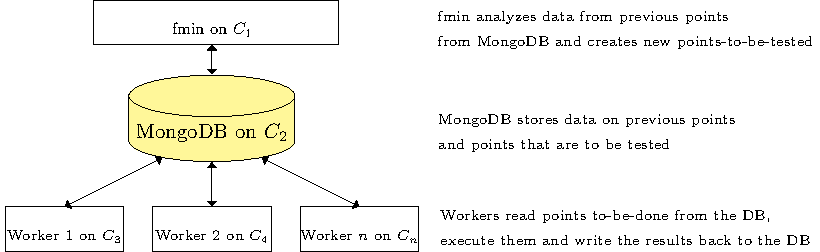
\includegraphics[width=0.7\paperwidth]{aufbau/aufbau.pdf}
        \caption{A simplified view of the OmniOpt is set up.}
\end{figure}

\subsection{Create a new optimization-project}

\subsubsection{Preparations for your program}

Before practically using OmniOpt, you need to prepare your program so that it runs on Taurus. That is,
you need to write a \ctexttt{bash}-file\footnote{Using \ctexttt{bash} is optional, but recommended; 
you can use any programming language you like.} that loads the modules you need. This might look like this:

\begin{lstlisting}[language=bash]
#!/bin/bash -l
# gets the path of the script to be run
module load modenv/scs5 # loads the appropriate modules
module load TensorFlow
python3 /path/to/yourprogram.py $1 $2 $3 $4 $5
# loads your program with 5 parameters that can be run like
# $ run.sh 1 2 3 4 5
\end{lstlisting}

The parameters \ctexttt{\$1}, \ctexttt{\$2} etc. can, for example, be the number of layers of a neural network,
or the number of neurons per layer or something like that.

\subsubsection{Define output values}

To be able to minimize any value, you have to specify what value the program returns (in the
analogy of $f(x_1, x_2, x_3, \dots) = y$, it's the $y$-value). This is easily done by
outputting 

\begin{cverbatim}
RESULT: 3.14159
\end{cverbatim}

somewhere in your program, to \ctexttt{STDOUT} (in most programming languages, this is done with
a \ctexttt{print}-statement). You can have as many of those outputs as you like, they'll all be saved
into the MongoDB-database, but the only one that can be optimized after is the \ctexttt{RESULT}-one,
thus, this is needed to run the program properly.

Instead of the values of $\pi$, you must, of course, output the
value you want to optimize (e.\,g. the loss of your neural network).

You can specify any number of values like

\begin{cverbatim}
e: 2.71828
c: 299792458
...
\end{cverbatim}

in the \ctexttt{STDOUT}-stream.

All of those will be parsed and saved into the \ctexttt{Mongo}-database (see section \ref{mongodb}) for later usage
and analysis.

You can also write your results to a file, but then, in the \ctexttt{bash}-file starting your script, read it after
it's run. Like 

\begin{lstlisting}[language=bash]
...
python3 /path/to/yourprogram.py $1 $2 $3 $4 $5
echo "RESULT: $(cat file_with_results.txt)"
\end{lstlisting}

As long as the `\ctexttt{RESULT}'-output exists and is somewhere in the whole \ctexttt{STDOUT} of the script,
it will work.

If there are multiple `\ctexttt{RESULT}'-outputs, only the last one will be saved!

\subsubsection{Via the GUI}

The recommended way of creating a new project is to use the GUI available under \url{https://imageseg.scads.de/omnioptgui/}.
It should be quite intuitive and does not allow for invalid parameters to be entered. It also allows the installation of
OmniOpt via an installer-script that is automatically generated.

\subsubsection{Manually}

\paragraph{Getting OmniOpt}

OmniOpt's source code must first be cloned from the global repository, which always contains the latest version.
First, \ctexttt{cd} into the folder that you want OmniOpt to be installed in, then:

\begin{lstlisting}[language=bash]
git clone --depth=1 file:///projects/p_scads/nnopt/bare/ .
\end{lstlisting}

\paragraph{Creating a new project}

Inside the OmniOpt-main-folder, there's a folder called ``projects''. Inside of this folder, create a new
folder that's named after your project. Please don't use spaces or other weird characters, but only
plain ASCII-characters without spaces when naming of that folder.

If you do not want to use this folder, but some other folder, this is possible, too. Create a folder that
is somehow accessible to OmniOpt from your user account and start the 
\ctexttt{sbatch.pl} with the parameter \ctexttt{$--$projectdir=/path/to/your/projects/}.

Inside of that folder, please create a pure text-file called ``\ctexttt{config.ini}'' (see \ref{configini})
and a folder called ``\ctexttt{program}'', in which you put your program's files.

Everything else will be created automatically.

\subsubsection{The \ctexttt{config.ini}-file}
\label{configini}

The \ctexttt{config.ini} is the main source for configuring the to-be-optimized job. It contains all the information needed
to run OmniOpt.

Here is an example \ctexttt{config.ini}-file for reference, of which I will go through all the lines to explain what they do
and how things can be set.

\begin{lstlisting}[language=Ini]
# Comments start with a hash sign
[DATA]
precision = 5
max_evals = 5000
objective_program = bash /your/omniopt/installation/projects/yourproject/program/run.sh int($x_0) int($x_1) ($x_2)
algo_name = tpe.suggest
range_generator_name = hp.uniform

[DIMENSIONS]
dimensions = 3

dim_0_name = epochs
min_dim_0 = 300
max_dim_0 = 330

dim_1_name = batchsz
range_generator_1 = hp.randint
max_dim_1 = 100

dim_2_name = nodes1
range_generator_2 = hp.choice
options_2 = 2,5,6,11

[DEBUG]
debug_xtreme = 1
debug = 1
info = 1
warning = 1
success = 1
stack = 0

[MONGODB]
worker_last_job_timeout = 500
poll_interval = 1
kill_after_n_no_results = 100
\end{lstlisting}

\paragraph{\ctexttt{[DATA]}}

The \ctexttt{[DATA]}-section contains information about the program and it's general settings. 

The \ctexttt{precision}-parameter controls how many digits after the decimal point should be shown. Generally, a value
of 2 or 3 should suffice.

The \ctexttt{max\_evals}-parameter contains the number of maximal runs the OmniOpt should try before giving up finding
a better minimum.

The \ctexttt{objective\_program}-parameter contains the path to the program that should be run. 
\ctexttt{\$x\_0}, \ctexttt{\$x\_1} etc. are the parameters that are given to the script (e.\,g.
$ f(\underbrace{x_0, x_1, x_2, \dots}_{\mathrm{These}}) $ in the analogy used before). The \ctexttt{int} around those is optional,
but guarantees that there are only integer values passed to the script, no matter of the algorithm chosen. Even without the \ctexttt{int}
around, there have to be brackets around the \ctexttt{(x\_n)}-values, so that it is always clear where a parameter starts and ends.

\ctexttt{algo\_name} chooses the algorithm which should be used for generating the
numbers\footnote{Check \url{https://conference.scipy.org/proceedings/scipy2013/pdfs/bergstra_hyperopt.pdf}
for more information, see especially page 14f.}.

\ctexttt{range\_generator\_name} chooses the algorithm which should be used for generating the ranges\footnote{Check \url{https://conference.scipy.org/proceedings/scipy2013/pdfs/bergstra_hyperopt.pdf}
for more information, see especially page 15f.}.

\paragraph{\ctexttt{[DIMENSIONS]}}

In this section, you can specify the so-called dimensions (the number of values that are passed to each script). Parameters:

\ctexttt{dim\_\textit{x}\_name} specifies the name for this specifix axis. \ctexttt{dim\_0\_name} is, in this example, ``epochs''.

\ctexttt{min\_dim\_0} and \ctexttt{max\_dim\_0} specify the range, in which the dimension 0 should be tried out. In this example, $ 300 < \mathrm{dim_0} < 350 $.
Instead of $0$, please use the appropriate dimension-number (starting with 0). If no range generator name is specified 
(e.\,g. with ``\ctexttt{range\_generator\_0}''), then the range generator of ``\ctexttt{range\_generator\_name}''
from the \ctexttt{[DATA]}-section is used. Other range generators may need other parameters. For example, \ctexttt{hp.randint} only needs a \ctexttt{max\_dim\_1}, but no \ctexttt{min\_dim\_1}.
The algorithm ``\ctexttt{hp.choice}'' chooses from a preselected list of options, in the above example it's $ \left\{\ctexttt{2, 5, 6, 11 }\right\} $.

\paragraph{\ctexttt{[DEBUG]}} --- This section enables different debugging options. If set to 0, it's disabled, and if it's 1, it's enabled.
None of these options are neccessary to turn on, except you want or need to debug errors.

\paragraph{\ctexttt{[MONGODB]}} --- In this, you can specify options for MongoDB. 

``\ctexttt{worker\_last\_job\_timeout}'' specifies after how many seconds of doing nothing a worker should be killed. 
Similiary, ``\ctexttt{kill\_after\_n\_no\_results}'' kills a worker after it had nothing to do $n$ times. The variable
''\ctexttt{poll\_interval}'' specifies how often the worker should look into the MongoDB for new jobs.

\subsection{Starting the jobs}

Once the project is set up, you can start a job with this simple bash command on Taurus.

\begin{lstlisting}[language=bash]
sbatch -J 'OmniOptProject' --mem-per-cpu='4096' --ntasks='5' \
--tasks-per-node=1 -p hpdlf --gres=gpu:1 --time="100:00:00" \
sbatch.pl --projectdir=/home/user/projects/
\end{lstlisting}

The \ctexttt{sbatch.pl} accepts the parameter \ctexttt{$--$project=projectname}, but it is not required, as long as
the Slurm-Job-Name is equal to the project name. The above command will, for example, start 5 workers with 1 GPU
for each worker on the \ctexttt{hpdlf} for 100 hours and with 4GB of RAM each. It will then optimize the \ctexttt{OmniOptProject}
that resides in \ctexttt{/home/user/projects/OmniOptProject}.

OmniOpt does not care whether you run it on a \ctexttt{x86\_64} or \ctexttt{PowerPC}-node (e.\,g. \ctexttt{ML}). It will automatically
load the proper modules. But make sure your own program works on the desired platform.

\subsection{Accessing the results}
%\label{mongodb}

\subsubsection{\ctexttt{bash dostuff.sh}}

The most convienent way of accessing almost all functions that OmniOpt offers is to use the command:

\begin{lstlisting}[language=bash]
bash dostuff.sh
\end{lstlisting}

This offers a CLI-based GUI that allows almost all commands that OmniOpt offers to be run without having to remember
any commands.

\begin{figure}[h!]
        \centering
        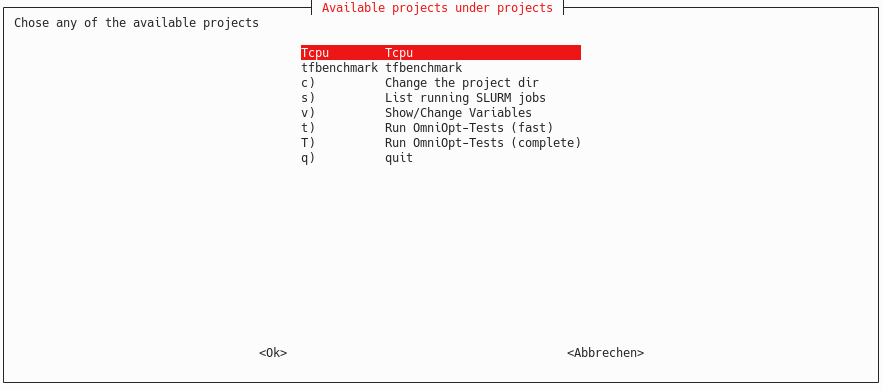
\includegraphics[width=0.7\paperwidth]{dostuff.png}
	\caption{The main screen of the \ctexttt{dostuff.sh}}
        \label{plotscreen}
\end{figure}

These include, but are not limited to, showing the plots from \ref{plot}, showing plots of GPU-usage, exporting
data to CSV, exporting videos of the database slowly `filling', running OmniOpt's extensive test-suite, getting
the wallclock-time of jobs and managing running slurm-jobs.

\subsubsection{Showing your results graphically}
\label{plot}

\begin{figure}[h!]
        \centering
        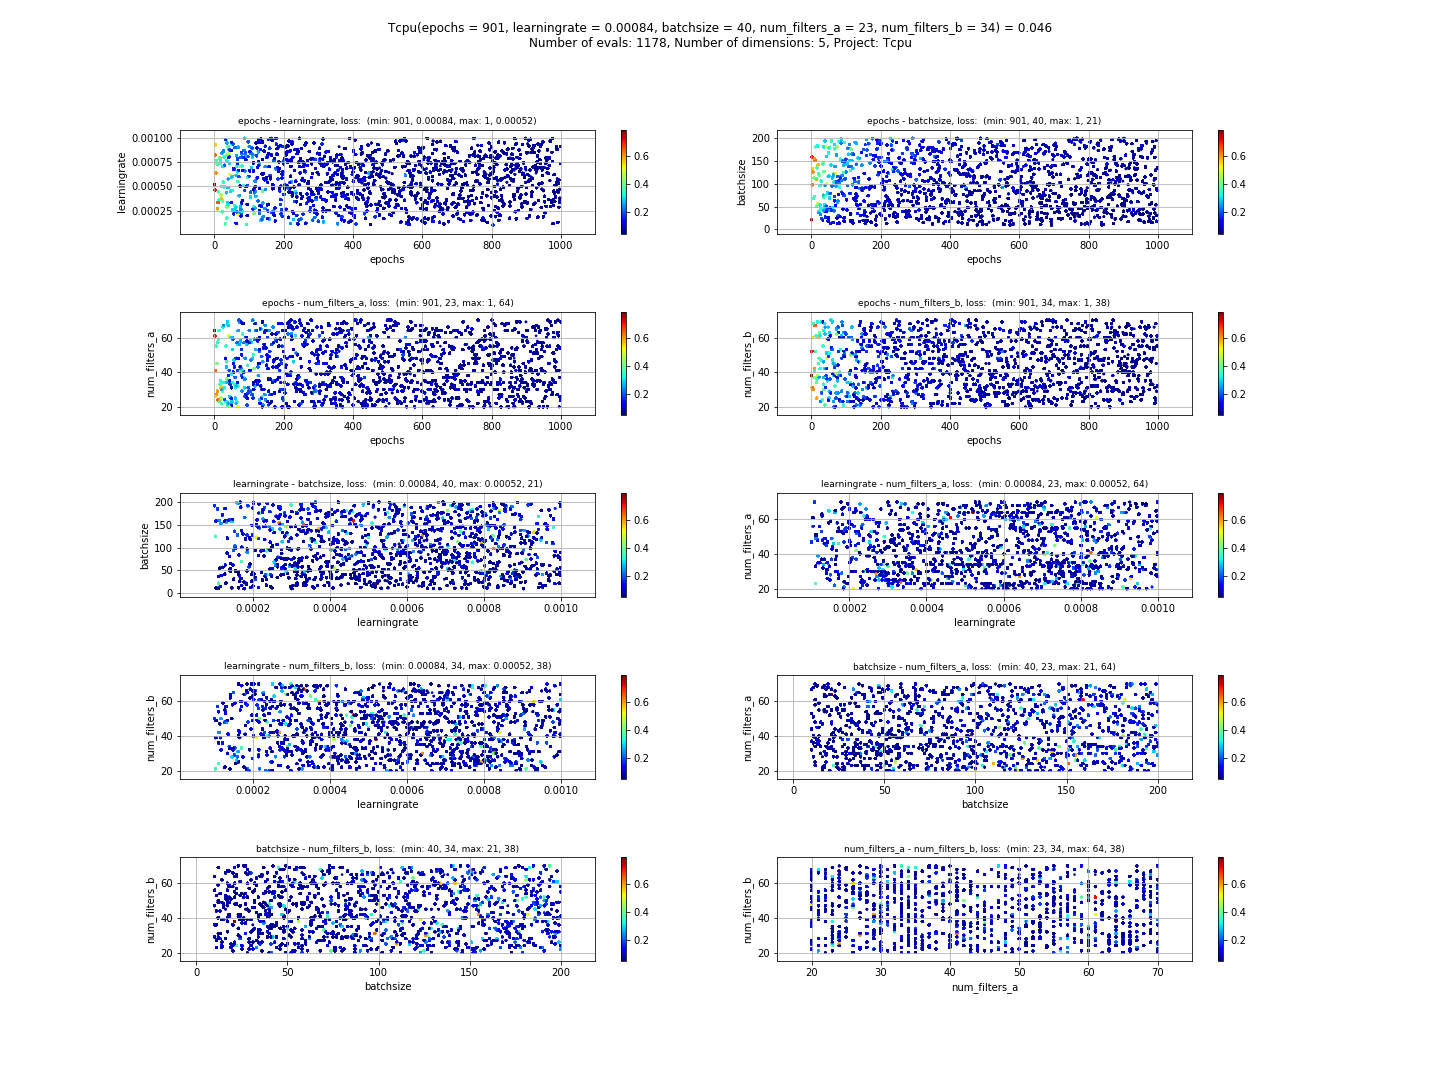
\includegraphics[width=0.7\paperwidth]{graph.png}
        \caption{The $n$-dimensional graph of a job (in this case with 5 dimensions, there are 10 sub-graphs, which can be calculated with $\left(n\atop 2\right)$).}
        \label{plotscreen}
\end{figure}

If you connect with \ctexttt{ssh -X} to Taurus, with the command

\begin{lstlisting}[language=bash]
bash tools/plot.sh --project=PROJECTNAME
\end{lstlisting}

you will get a screen like the one in figure \ref{plotscreen}. There, you'll see all permutations of the axis that you can put together to
an $n$-dimensional picture in your head. Here, dimension-names also become important, so you can see where which dimension is easily. 

Each colored dot is one run of the job, and the ``bluer'' it is, the better it's value is. If, for example, a lot of blue dots are on the
right side of one specific axis, you can guess that it might be useful to increase that axis' maximum value, so a better minimum might be
found there.


\subsubsection{Get runtimes of your program with statistics}

With the program \ctexttt{analyze\_log\_file.pl} you can get statistical data about OmniOpt-jobs that already ran.
All you need is the slurm-log-file in the same directory as the \ctexttt{analyze\_log\_file.pl} and this command:

\begin{lstlisting}[language=bash]
module load modenv/classic
module load mongodb/3.6.3
perl tools/analyze_log_file.pl --slurmid=6740000
\end{lstlisting}

This will take some time, because it will start the appropriate MongoDB-process for this log-file's projectname
in the background and analyze it's data. You will get an output similiar to this:

\begin{cverbatim}
Slurm-ID: 6740000 | Project: bm60_3 | Workers: 60 | 
Runtime (Slurm): 10:00:09 | Runtime (DB): 00:59:59 | 
Jobs done: 4711 | Avg. runtime/J (DB): 00:59:59 | 
J/s (Slurm): 0.13 | Job done every s (Slurm): 7.69
\end{cverbatim}

It distinguishes between Slurm-Time and DB-time, because sometimes the workers are idle and are not actually working,
because, for example, all the jobs are finished. So that the ``Jobs per second'' time is different, regarding whether you
use the real-used-time, or the time the slurm-job ran.

With the command \ctexttt{-{}-csv} you will get even more outputs, including the $x_1, x_2, x_3, \dots$-values of the 
run with the minimal ``RESULT'', all sourted in a CSV-file.

\begin{lstlisting}[language=bash]
perl tools/analyze_log_file.pl --slurmid=6740000 --csv
\end{lstlisting}


If this command fails, you can check the output of the \ctexttt{-{}-debug} parameter, which shows every step taken to get to
the results. Whenever the database couldn't be started (e.\,g. because it's already running, or it is corrupt or something
else), some values will be negative.

\subsubsection{Accessing the database}

Once the job ran, you can access it's database. With the script

\begin{lstlisting}[language=bash]
python3 script/startmongodb.py --project=PROJECTNAME
\end{lstlisting}

the database will automatically start on the folder of the specified project name. In this, you can now view the data
as you would normally do in MongoDB.

It will print some lines like

\begin{cverbatim}
mongodb://127.0.0.1:4324/bm1
\end{cverbatim}

These lines you can use to connect to the DB with

\begin{cverbatim}
mongo mongodb://127.0.0.1:4324/bm1
\end{cverbatim}

Inside the Mongo-Shell, you can then go to the database of the project with 
\begin{lstlisting}[language=JavaScript]
use PROJECTNAME;
db.jobs.find({}, {}).pretty();
\end{lstlisting}

If there's an error like ``\ctexttt{The file `bm1/mongodb/mongod.lock` already exists!!!}'',
please check that there are no running processes and of this MongoDB instance and then just delete this lock-file and restart the process.

\section{Debugging}

\subsection{\ctexttt{module: command not found}, \ctexttt{ml: command not found}}

When you're loading many workers that are on different nodes, it seems as if the Slurm-daemon tries to connect to
the worker via \ctexttt{ssh} via a non-interactive shell. This way, \ctexttt{/etc/profile.d/} does not get loaded.

Because of that, the shell-program \ctexttt{module} also does not get loaded. Force the script to use the profiles-folder
by using: \ctexttt{\#!/bin/bash -l} as shebang in the first line.

\subsection{Slurm-Output-files}

Lots of things are getting logged automatically, so you can always check when something goes wrong. The logs are in various places
where you can go and look for them. The main place for logs that are done when running a slurm-job is whereever OmniOpt was 
installed to . There, jobs with names like \ctexttt{slurm-6739996.out} are saved.

You can access those logs after a job has been finished, or while it is running with

\begin{lstlisting}[language=bash]
tail -f slurm-6739996.out
\end{lstlisting}

so you can see it's output live, as they appear.

\subsection{See the output of every worker}

In the \ctexttt{projects}-folder of a project, after a job has been started, there's a folder
called \ctexttt{logs}. Inside this folder, there are other folders, one for every job started, with the time the main-job has started, and
inside if this, there's one log-file for every worker that ran on that specific job.

To see the outputs of the programs themselves, see: \ctexttt{projects/\$PROJECTNAME/program.log}. Inside these log files, 
there are all the outputs of that one specific worker-slurm-subprocess.

\end{document}
